\makeatletter
\providecommand{\bigsqcap}{%
  \mathop{%
    \mathpalette\@updown\bigsqcup
  }%
}
\newcommand*{\@updown}[2]{%
  \rotatebox[origin=c]{180}{$\m@th#1#2$}%
}
\makeatother

\makeatletter
\let\oldnl\nl% Store \nl in \oldnl
\newcommand{\nonl}{\renewcommand{\nl}{\let\nl\oldnl}}% Remove line number for one line
\makeatother

\let\oldalgorithm\algorithm
\let\oldendalgorithm\endalgorithm

  \let\algorithm\figure
  \let\endalgorithm\endfigure

\chapter{Design}
\label{chapter:Design}

In the design of \textit{TypeShield}, we cover various aspects, first of all we present the details of the 
\emph{count} policy in Section \ref{section:countpolicy} - as introduced by \cite{veen:typearmor} - 
and the new \emph{type} policy in Section \ref{section:typepolicy}. Then we describe general 
theory needed to transform set-based analyses to register based ones in Section \ref{section:instructionanalysis}. 
We follow this up by presenting the theory needed  implement the analysis for calltargets  in 
Section \ref{section:calltargetanalysis} and  callsites in Section \ref{section:callsiteanalysis} 
for each policy. Finally, in Section \ref{section:addresstakenanalysis} we introduce a version of 
address taken analysis based on \cite{mingwei:sekar} to restrict the number of available calltargets even more. 
%At last we introduce a patching schema for callsites and calltargets to enforce the invariants we inferred.

\section{\emph{Count} Policy}
\label{section:countpolicy}

What we call the \emph{count} policy is essentially the policy introduced by TypeArmor \cite{veen:typearmor}. 
The basic idea revolves aroung classifying calltargets by the number of parameters they provide and callsites 
by the number of paramters they require. The schema to match those is that we have calltargets requiring 
parameters and the callsites providing parameters as depicted in Figure \ref{fig:COUNTschema}.

\begin{figure}[!h]
\centering
\resizebox{0.80\textwidth}{!}{
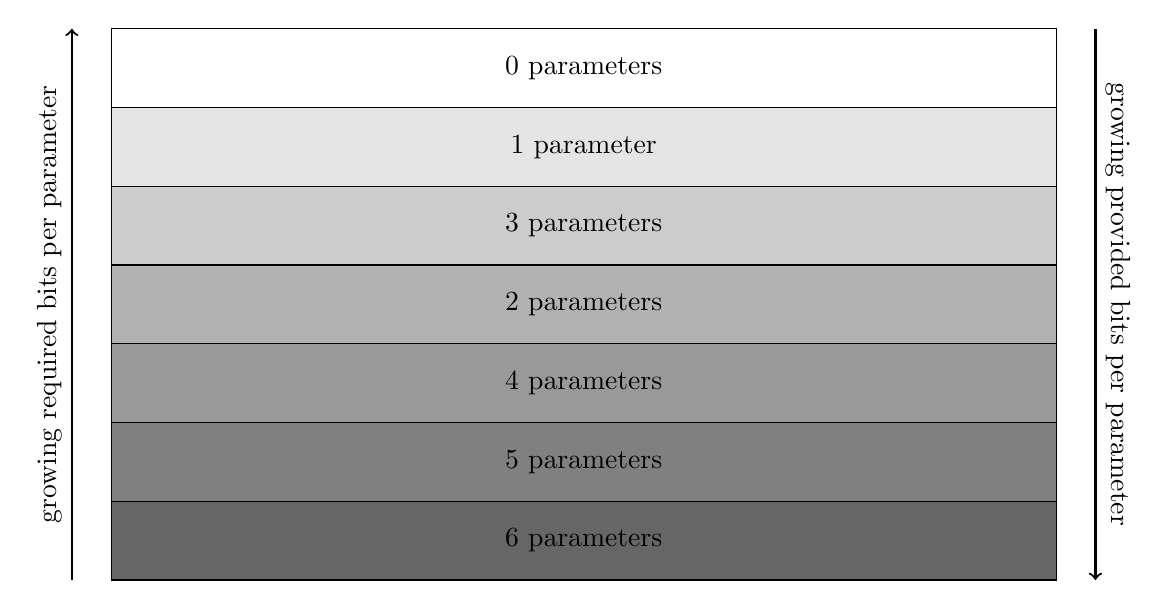
\begin{tikzpicture}

%\fill[black!40!white] (0,0) rectangle (9,9);
%\fill[black!30!white] (0,0) rectangle (7,7);
%\fill[black!20!white] (0,0) rectangle (4,4);
%\fill[black!10!white] (0,0) rectangle (2,2);
%
%\draw (0,0) --node[anchor=south] {0 params}  (2,0)  -- (2,2) -- (0,2) -- (0,0) ;
%\draw (0,0) -- (2,0) --node[anchor=south] {1 param} (4,0) -- (4,4) -- (0,4) -- (0,0);
%\draw (0,0) --(4,0) --node[anchor=south] {2 ... 5 params} (7,0) -- (7,7) -- (0,7) -- (0,0);
%\draw (0,0) --(7,0) --node[anchor=south] {6 params} (9,0) -- (9,9) -- (0,9) -- (0,0);
%\draw[dashed] (4,4) -- (7,7);


\fill[black!00!white] (0,7) rectangle (12,6);
\fill[black!10!white] (0,6) rectangle (12,5);
\fill[black!20!white] (0,5) rectangle (12,4);
\fill[black!30!white] (0,4) rectangle (12,3);
\fill[black!40!white] (0,3) rectangle (12,2);
\fill[black!50!white] (0,2) rectangle (12,1);
\fill[black!60!white] (0,1) rectangle (12,0);


\draw[thick,->] (-0.5,0) -- node[sloped, anchor=center, above] {growing required bits per parameter} (-0.5,7);
\draw[thick,->] (12.5,7) -- node[sloped, anchor=center, above] {growing provided bits per parameter} (12.5,0);

\draw (0,7) rectangle node[anchor=center] {0 parameters} (12,6);

\draw (0,6) rectangle node[anchor=center] {1 parameter} (12,5);

\draw (0,5) rectangle node[anchor=center] {3 parameters} (12,4);

\draw (0,4) rectangle node[anchor=center] {2 parameters} (12,3);

\draw (0,3) rectangle node[anchor=center] {4 parameters} (12,2);

\draw (0,2) rectangle node[anchor=center] {5 parameters} (12,1);

\draw (0,1) rectangle node[anchor=center] {6 parameters} (12,0);


\end{tikzpicture}
}
\caption{\emph{Count} policy classification schema for callsites and calltargets.}
\label{fig:COUNTschema}
\end{figure}

 Furthermore, generating 100\% precise measurements for such classification with binaries as the only source of information is rather difficult. Therefore overestimations of parameter count for callsites and underestimations of the parameter count for calltargets is deemed acceptable. This classification is based on the general purpose registers that the call convention of the current ABI - in this case the SystemV ABI - designates as parameter registers. Furthermore, we completely ignore floating point registers or multiinteger registers. The core of the \emph{count} policy is now to allow any callsite $cs$, which provides $c_{cs}$ parameters, to call any calltarget $ct$, which requires $c_{ct}$ parameters, iff $c_{ct} \leq c_{cs}$ holds. However, the main problem is that while there is a significant restriction of calltargets for the lower callsites, the restriction capability drops rather rapidly when reaching higher parameter counts, with callsites that use 6 or more parameters being able to call all possible calltargets:
\[
	\forall cs_1, cs_2.  c_{cs_1} \leq c_{cs_2} \Longrightarrow  \| \{ct \in \mathcal{F} | c_{ct} \leq c_{cs_1} \} \| \leq \| \{ct \in \mathcal{F} | c_{ct} \leq c_{cs_2}  \} \|
\]
One possible remedy would be the ability to introduce an upper bound for the classification deviation of parameter counts, however as of now, this does not seem feasible with current technology. Another possibility would be the overall reduction of callsites, which can access the same set of calltargets, a route we will explore within this work.

\section{\emph{Type} Policy}
\label{section:typepolicy}

What we call the \emph{type} policy is the idea of not only relying on the parameter count but also on the type of a parameter. However due to complexity reasons, we are restricting ourselves to the general purpose registers, which the SystemV ABI designates as parameter registers. Furthermore we are not inferring the actual type of the data but the wideness of the data stored in the register. The schema again is that we have calltargets requiring wideness and the callsite providing 
wideness as depicted in Figure \ref{fig:TYPEschema}.
\begin{figure}[!h]
\center
\resizebox{0.75\textwidth}{!}{
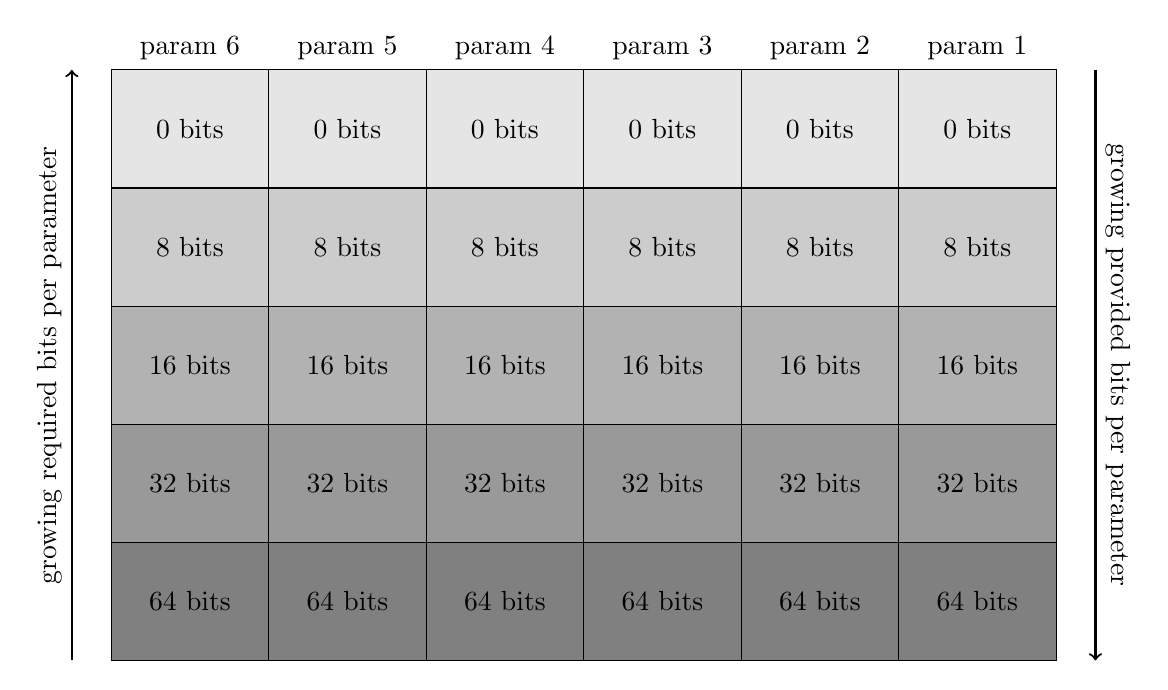
\begin{tikzpicture}

\fill[black!10!white] (0,7.5) rectangle (12,6);
\fill[black!20!white] (0,6) rectangle (12,4.5);
\fill[black!30!white] (0,4.5) rectangle (12,3);
\fill[black!40!white] (0,3) rectangle (12,1.5);
\fill[black!50!white] (0,1.5) rectangle (12,0);

\draw[thick,->] (-0.5,0) -- node[sloped, anchor=center, above] {growing required bits per parameter} (-0.5,7.5);
\draw[thick,->] (12.5,7.5) -- node[sloped, anchor=center, above] {growing provided bits per parameter} (12.5,0);

\draw (0,7.5) --node[anchor=south] {param 6} (2,7.5);
\draw (2,7.5) --node[anchor=south] {param 5} (4,7.5);
\draw (4,7.5) --node[anchor=south] {param 4} (6,7.5);
\draw (6,7.5) --node[anchor=south] {param 3} (8,7.5);
\draw (8,7.5) --node[anchor=south] {param 2} (10,7.5);
\draw (10,7.5) --node[anchor=south] {param 1} (12,7.5);

\draw (0,7.5) rectangle node[anchor=center] {0 bits} (2,6);
\draw (2,7.5) rectangle node[anchor=center] {0 bits} (4,6);
\draw (4,7.5) rectangle node[anchor=center] {0 bits} (6,6);
\draw (6,7.5) rectangle node[anchor=center] {0 bits} (8,6);
\draw (8,7.5) rectangle node[anchor=center] {0 bits} (10,6);
\draw (10,7.5) rectangle node[anchor=center] {0 bits} (12,6);

\draw (0,6) rectangle node[anchor=center] {8 bits} (2,4.5);
\draw (2,6) rectangle node[anchor=center] {8 bits} (4,4.5);
\draw (4,6) rectangle node[anchor=center] {8 bits} (6,4.5);
\draw (6,6) rectangle node[anchor=center] {8 bits} (8,4.5);
\draw (8,6) rectangle node[anchor=center] {8 bits} (10,4.5);
\draw (10,6) rectangle node[anchor=center] {8 bits} (12,4.5);

\draw (0,4.5) rectangle node[anchor=center] {16 bits} (2,3);
\draw (2,4.5) rectangle node[anchor=center] {16 bits} (4,3);
\draw (4,4.5) rectangle node[anchor=center] {16 bits} (6,3);
\draw (6,4.5) rectangle node[anchor=center] {16 bits} (8,3);
\draw (8,4.5) rectangle node[anchor=center] {16 bits} (10,3);
\draw (10,4.5) rectangle node[anchor=center] {16 bits} (12,3);

\draw (0,3) rectangle node[anchor=center] {32 bits} (2,1.5);
\draw (2,3) rectangle node[anchor=center] {32 bits} (4,1.5);
\draw (4,3) rectangle node[anchor=center] {32 bits} (6,1.5);
\draw (6,3) rectangle node[anchor=center] {32 bits} (8,1.5);
\draw (8,3) rectangle node[anchor=center] {32 bits} (10,1.5);
\draw (10,3) rectangle node[anchor=center] {32 bits} (12,1.5);

\draw (0,1.5) rectangle node[anchor=center] {64 bits} (2,0);
\draw (2,1.5) rectangle node[anchor=center] {64 bits} (4,0);
\draw (4,1.5) rectangle node[anchor=center] {64 bits} (6,0);
\draw (6,1.5) rectangle node[anchor=center] {64 bits} (8,0);
\draw (8,1.5) rectangle node[anchor=center] {64 bits} (10,0);
\draw (10,1.5) rectangle node[anchor=center] {64 bits} (12,0);
\end{tikzpicture}
}

\caption{\emph{Type} policy schema for callsites and calltargets.}
\label{fig:TYPEschema}
\end{figure}

We are currently interested in x86-64 binaries, the registers we are looking at are 64bit registers that can be accessed in 4 different ways:
\begin{itemize}
\item the whole 64bits of the register, meaning a wideness of 64.
\item the lower 32bits of the register, meaning a wideness of 32.
\item the lower 16bits of the register, meaning a wideness of 16.
\item the lower 8bits of the register, meaning a wideness of 8.
\end{itemize}

Four of those registers can also directly access the higher 8bits of the lower 16bits of the register. For our purpose we register this access as a 16bit access. Based on this information, we can assign a register one of 5 possible types $\mathcal{T} = \{64, 32, 16, 8, 0\}$. We also included the type 0 to model the absence of data within a register. Similar to the \emph{count} policy, we allow overestimation of types in callsites and underestimation of types in calltargets. However, the matching idea is different, 
because as can we depict in Figure \ref{fig:TYPEschema}, the type of a calltarget and a callsite no longer depends solely on its parameter count, each callsite and calltarget has its type from the set of $\mathcal{T}^6$, with the following comparison operator:
\[
	u \leq_{type} v :\Longleftrightarrow  \forall_{i = 0}^{5} {u_i \leq v_i} , \text {with } u, v \in \mathcal{T}^6
\]
Again we allow any callsite $cs$ call any calltarget $ct$, when it fulfills the requirement $ct \leq cs$. The way we represent this is by letting the type for a calltarget parameter progress from 64bit to 0bit - If a calltarget requires a 32bit value in its 1st parameter, it also should accept a 64bit value from its callsite - and similarly we let the type for a callsite progress from 0bit to 64bit - If a callsite provides a 32bit value in its 1st parameter it also provides a 16bit, 8bit and 0bit to a calltarget. Now the advantage of the \emph{type} policy in comparison to the \emph{count} policy is that while our type comparison implies the count comparison, the other direction does not hold. Meaning, just having an equal or lesser number of parameters than a callsite, does no longer allow a calltarget being called there, thus restricting the number of calltargets per callsite even further. A function that requires 64bit in its first parameter, and 0bit in all other parameters, would have been callable by a callsite providing 8bit in its first and second parameter when using the \emph{count} policy, however in the \emph{type} policy this is no longer possible.


\section{Instruction Analysis}
\label{section:instructionanalysis}
Usually data-flow analysis algorithms are based on set of variable or sets of definitions, which both are basically unbounded. However, we are analysing the state of registers, which are baked into hardware and therefore their number is given, thus requiring us to adapt the data-flow theory to work on tuples.

The set $\mathcal{I}$ describes all possible instructions that can occur within the executable section of a binary. (in our case this is based on the instruction set for x86-64 processors)

An instruction $i \in \mathcal{I}$ can non-exclusively perform two kinds of operations on any number of existing registers:

\begin{enumerate}
\item Read $n$ bits from the register with $n \in \{ 64, 32, 16, 8 \}$.
\item Write $n$ bits to the register with $n \in \{ 64, 32, 16, 8 \}$.
\end{enumerate}

Thus we describe the possible change that occurs in one register with the set $S = \{ w64, w32, w16, w8, 0 \} \times \{r64, r32, r16, r8, 0 \}$. Note that 0 signals the absence of either a write or read access and $(0, 0)$ signals the absence of both. Furthermore $wn$ or $rn$ with $n \in \{64,32,16,8\}$ implies all $wm$ or $rm$ with $m \in \{64,32,16,8\}$ and $m < n$ (e.g. $r64$ implies $r32$). Note that we exclude 0, as it means the absence of any access.

SystemV ABI specifies 16 general purpose integer registers, thus for our purpose we represent the change occurring at the processor level as $\mathcal{S} = S^{16}$.

At last we declare a function, which calculates the change occurring in the processor state, when executing an instruction from $\mathcal{I}$:
\[
decode : \mathcal{I} \mapsto \mathcal{S}
\]

However, we do not go into detail how this function actually calculates this sate, because we rely on external libraries to perform this task. Implementing this function ourself is out of scope due to the lengthy work required, as the x86-64 instruction set is quite large.

\section{Calltarget Analysis}
\label{section:calltargetanalysis}
For either \emph{count} or \emph{type} policy to work, we need to arrive at an underestimation of the required parameters by any function existing within the targeted binary. We will employ a modified version of liveness analysis that tracks registers instead of variables to generate the needed underestimation. As our algorithm will be customizable, we look at the required merge functions to implement \emph{count} and \emph{type} policy. Furthermore we need to eliminate the passing of variadic parameter lists from variadic functions, as this might cause our analysis to overestimate the required parameters.

\subsection{Variable Liveness Analysis Theory}
\label{subsection:livenessanalysis}
A variable is alive before the execution of an instrucction, if at least one of the originating paths contains a read access before the variable is written to again. We employ liveness analysis, because we are looking for the  parameters a function requires. This essentially requires read before write access, however global variables usually would also fall into this category, however these would not reside within parameter registers at the start of a function.

The book ``Data Flow Analysis - Theory and Practice'' \cite{khedker2009data} defines live variable analysis on blocks in the following manner:

\begin{center}
\begin{subequations}
\label{eq:livenessbasedef}
\begin{align}
In_n &:= (Out_n - Kill_n) \cup Gen_n \label{eq:livenessbasedefIn} \\
Out_n &:= \left\{
  \begin{array}{lr}
    Bl & \text{n is end block}\\
    \underset{s \in succ(n)}{\bigcup} In_s & \text{otherwise}
  \end{array}
\right. \label{eq:livenessbasedefOut}
\end{align}
\end{subequations}
$Bl$ is the default state at the end of a path of execution and in our case reaching that state would mean that a variable has never been used (neither written nor read). The set $Kill_n$ describes all variables that are no longer live after the block $n$, meaning that a variable occurring within this set has been written to. The set $Gen_n$ describes all variables that are alive due to the block $n$, meaning that a variable occurring within this set has been read before it was written to.

\begin{algorithm}[!h]
	\SetAlgoLined
	\SetKwProg{Fn}{Function}{ is}{end}
	\Fn{analyze(block : BasicBlock) : $\mathcal{S}^\mathcal{L}$}
	{
 	state = Bl
 	
 	\ForEach{inst $\in$ block}{
 	
 		state' = analyze\_instr(inst)
 		
		state = merge\_v(state, state')
	}

	states = \{\}
	
	blocks = succ(block)
	
	\ForEach{block' $\in$ blocks} {
	
 		state' = analyse(block')
 		
		states = states $\cup$ \{ state' \}
	}

	state' = merge\_h (states)

	\Return merge\_v(state, state')

	}
\caption{Algorithm to analyse the liveness of a Basic Block.}
\label{alg:liveness}
\end{algorithm}
\end{center}

However, we cannot use variable liveness analysis as is, because the analysis is based on potentially unbound variable sets, while we are restricted to a finite number of registers and states. We also require an underestimation of live variables an not an overestimation as provided by standard liveness analysis. Furthermore we have to define how to interpret the changes occurring within one block based on the the change caused by its instructions. Considering this, we arrive at algorithm \ref{alg:liveness} to compute the liveness state at the start of a basic block.

This algorithm relies on various functions that can be used to configure its behaviour. We need to define the function $merge\_v$, which describes how to compound the state change of the current instruction and the current state, the function $merge\_h$, which describes how to merge the states of several paths, the instruction analysis function $analyze\_instr$. The function $succ$, which retrieves all possible successors of a block won't be implemented by us, because we rely on the DynInst instrumentation framework to achieve this.

\begin{subequations}
\label{eq:livenesscustom}
\begin{align}
merge\_v &: \mathcal{S}^\mathcal{L} \times \mathcal{S}^\mathcal{L} \mapsto \mathcal{S}^\mathcal{L}\\
merge\_h &: \mathcal{P}(\mathcal{S}^\mathcal{L}) \mapsto \mathcal{S}^\mathcal{L}\\
analyze\_instr &: \mathcal {I} \mapsto \mathcal{S}^\mathcal{L} \\
succ &: \mathcal{I} \mapsto \mathcal{P}(\mathcal{I})
\end{align}
\end{subequations}

%\begin{subequations}
%\label{eq:livenesscustom}
%\begin{align}
%In_n &:= merge\_v(n, Out_n)\label{eq:livenesscustomIn} \\
%Out_n &:= \left\{
%  \begin{array}{lr}
%    Bl & \text{n has no successors}\\
%    merge\_h( \{ In_s | s \in succ(n) \} & \text{otherwise}
%  \end{array}
%\right. \label{eq:livenesscustomOut}\\
%merge\_v &: \mathcal{I} \times \mathcal{S}^\mathcal{L} \mapsto \mathcal{S}^\mathcal{L}\\
%merge\_h &: \mathcal{P}(\mathcal{S}^\mathcal{L})  \mapsto \mathcal{S}^\mathcal{L}\\
%succ &: \mathcal{I} \times \mathcal{P}(\mathcal{I})
%\end{align}
%\end{subequations}
%We have yet to define the functions $merge\_v$, which describes how to compound a function and the outgoing state, the function $merge\_h$, which describes how to merge the states of several paths and the function $succc$, which essentially gives us the successors of the current instruction. To prevent cycles we keep track of the instructions visited within the current path and omit any instruction on the current path from the result of $succ$. These functions, the liveness state $\mathcal{S}^\mathcal{L}$ and its interpretation into parameters will be defined in the following subsections.

As the $analyze\_instr$ function calculates the effect of an instruction and is the heart of the analyze function. It will also handle non jump and non fallthrough successors, as these are not handled by DynInst in our case. We essentially have four cases that we handle:
\begin{enumerate}
\item if the instruction is an indirect call or a direct call but we chose not follow calls, then return a state where all registers are considered written.
\item if the instruction is a diect call and we chose to follow calls, then we spawn a new analysis and return its result.
\item if the instruction is a constant write (e.g. xor of two registers) then we remove the read portion before we return the decoded state.
\item in all other cases we simply return the decoded state
\end{enumerate}

This leaves us with the two merge functions remaining undefined and we will leave the implementation of these and the interpretation of the liveness state $\mathcal{S}^\mathcal{L}$ into parameters up to the following subsections.

\subsection{Required Parameter Count}
\label{subsection:requiredparamcount}

To implement the \emph{count} policy, we only need a coarse representation of the state of one register, thus we are interested in the following three different exclusive informations:
\begin{enumerate}
\item Was the register written to before its value could be read ? \\ We represent this with the state W.
\item Was the register read from before its value was overwritten ? \\ We represent this with the state R.
\item Did neither read nor write access occur for the register ? \\ We represent this with the state C.
\end{enumerate}
This gives us the following register state $S^\mathcal{L} = \{ C, R, W \}$ which translates to the register superstate $\mathcal{S}^\mathcal{L} = (S^\mathcal{L})^{16}$.
Now, we assume that unless the instructions we are looking at does discard the value it is reading (\texttt{xor rax rax} would be such an instruction that we call const\_write) that reading does preced the writing withing one instruction. Furthermore we are only interested in the first occurrence of a R or W within one path, as following reads or writes do not give us more information.
Therefore, we can define our vertical merge function in the following way:
\begin{align}
merge\_v^{r} (cur, delta) &= \left\{
  \begin{array}{lr}
     delta & cur = C \\
     cur & otherwise
  \end{array}
\right. \\
merge\_v (cur, delta) &= (s'_0, ... s'_15) \text { with } s'_j = merge\_v^{r}(cur_j, delta_j)
\end{align}


Our horizontal merge function is a simple pairwise combination of the given set of states:
\begin{align}
merge\_h(\{s\}) &= s\\
merge\_h(\{s\} \cup s') &= s \circ merge\_h(s')
\end{align}

We have three viable possibilities for our combination operator $\circ$, depicted in Table \ref{fig:COUNTlivenessmapping}, which all give priority to $W$:
\begin{itemize}
\item [$\bigsqcap^{\mathcal{L}}$] is what we call the destructive combination operator, as it returns W on any mismatch.
\item [$\bigcap^{\mathcal{L}}$] is what we call the intersection operator, as it returns C, when combining C and R, similar to an intersection.
\item [$\bigcup^{\mathcal{L}}$] is what we call the union operator, as it returns R, when combining C and R similar to a union.
\end{itemize}


\newcolumntype{?}{!{\vrule width 1pt}}

\begin{table}

\centering
\begin{tabular}{c?c|c|c}
$\bigsqcap^{\mathcal{L}}$ & C & R & W\\
\Xhline{1pt}
C & C & W & W\\
\hline
R & W & R & W\\
\hline
W & W & W & W
\end{tabular}
\begin{tabular}{c?c|c|c}
$\bigcap^{\mathcal{L}}$  & C & R & W\\
\Xhline{1pt}
C & C & C & W\\
\hline
R & C & R & W\\
\hline
W & W & W & W
\end{tabular}
\begin{tabular}{c?c|c|c}
$\bigcup^{\mathcal{L}}$  & C & R & W\\
\Xhline{1pt}
C & C & R & W\\
\hline
R & R & R & W\\
\hline
W & W & W & W
\end{tabular}


\caption{Different mappings for combining two liveness state values in horizontal matching for the \emph{count} policy.}

\label{fig:COUNTlivenessmapping}
\end{table}

We apply the liveness analysis for each function with the entry block of the function as start and the return blocks as end and after an analysis run for a function, the index of highest parameter register based on the used callconvention that has the state R is considered to be the number of parameters a function at least requires to be prepared by a callsite.


\subsection{Required Parameter Wideness}
\label{subsection:requiredparamwideness}
To implement the \emph{type} policy, we need a finer representation of the state of one register, thus we are interested in the following three different not neccessarily exlusive informations:
\begin{enumerate}
\item Was the register written to before its value could be read ? \\ We represent this with the state $W$.
\item How much was read from the register before its value was overwritten? \\ We represent this with the states $\{ r8, r16, r32, r64 \}$ using $R$ as a placeholder for arbitrary reads.
\item Did neither read nor write access occur for the register ? \\ We represent this with the state $C$.
\end{enumerate}
This gives us the following register state $S^\mathcal{L} = \{ C, r8, r16, r32, r64, W \}$ which translates to the register superstate $\mathcal{S}^\mathcal{L} = (S^\mathcal{L})^{16}$.
Now, we assume that unless the instructions we are looking at does discard the value it is reading (\texttt{xor rax rax} would be such an instruction that we call const\_write) that reading does preced the writing withing one instruction.

As there could happen more than one read of a register before it is written, we might be interested in more than just the first occurrence of a write or read on a path. We arrive therefore at three possible vertical merge functions:
\begin{itemize}
	\item The same vertical merge operator as used in the \emph{count} policy, which only gives us the first non $C$ state ($merge\_v^{r}$).
	\item A vertical merge operator that conceptually intersects all read accesses along a path until the first write occurs ($merge\_v^{i}$).
	\item A vertical merge operator that conceptually calculates the union of all read accesses along a path until the first write occurs ($merge\_v^{u}$).
\end{itemize}

Our horizontal merge function is a simple pairwise combination of the given set of states:
\begin{align}
merge\_h(\{s\}) &= s\\
merge\_h(\{s\} \cup s') &= s \circ merge\_h(s')
\end{align}

The results of our experiments with the implementation of calltarget classification gave presented us with essentially one possible candidate that we can base our horizontal merge function on, namely the union operator with an analysis function that follows into direct calls. The basic schema of the merging is depicted in \ref{tbl:TYPECTunion} and it essentially behaves as if it was the union operator (when both states are set, the higher one is chosen). However, we have to account for W being used as an end marker, which is why we added mapping for RW, which is essentially that. 

\begin{table}[h]
\centering
\begin{tabular}{c?c|c|c|c}
$\bigcup^{\mathcal{L}}$  & C & R & W & RW\\
\Xhline{1pt}
C & C & R & W & RW\\
\hline
R & R & $\text{R}^{\cup}$ & W & $\text{R}^{\cup}$W\\
\hline
W & W & W & W & W\\
\hline
RW & RW & $\text{R}^{\cup}$W & W & RW\\
\end{tabular}
\caption{The union mapping operator for liveness in the \emph{type} policy.}
\label{tbl:TYPECTunion}
\end{table}

\subsection{Variadic Functions}
\label{subsection:variadicfunctions}
Variadic functions are special functions in C/C++ that have a basic set of parameters, which they always require and a variadic set of parameters, which as the name suggests may vary. A prominent example of this would be the $printf$ function, which is used to output text to $stdout$.

The problem with these functions is that to allow for easier processing of parameters usually all potential variadic parameters are moved into a contiguous block of memory, as can be seen in the assembly in 
Figure \ref{fig:asmvariadic}. Our analysis interprets that as a read access on all parameters and we arrive at a problematic overestimation. 

\begin{figure}
\centering\begin{BVerbatim}
00000000004222f0 <make_cmd>:
  4222f0:       push   %r15
  4222f2:       push   %r14
  4222f4:       push   %rbx
  4222f5:       sub    $0xd0,%rsp
  4222fc:       mov    %esi,%r15d
  4222ff:       mov    %rdi,%r14
  422302:       test   %al,%al
  422304:       je     42233d <make_cmd+0x4d>
  422306:       movaps %xmm0,0x50(%rsp)
  42230b:       movaps %xmm1,0x60(%rsp)
  422310:       movaps %xmm2,0x70(%rsp)
  422315:       movaps %xmm3,0x80(%rsp)
  42231d:       movaps %xmm4,0x90(%rsp)
  422325:       movaps %xmm5,0xa0(%rsp)
  42232d:       movaps %xmm6,0xb0(%rsp)
  422335:       movaps %xmm7,0xc0(%rsp)
  42233d:       mov    %r9,0x48(%rsp)
  422342:       mov    %r8,0x40(%rsp)
  422347:       mov    %rcx,0x38(%rsp)
  42234c:       mov    %rdx,0x30(%rsp)
  422351:       mov    $0x50,%esi
  422356:       mov    %r14,%rdi
  422359:       callq  409430 <pcalloc>
\end{BVerbatim}
\caption{ASM code of the \texttt{make\_cmd} function with optimize level O2, which has a variadic parameter list.}
\label{fig:asmvariadic}
\end{figure}

Our solution to this problem is to find these spurious reads and ignore them. A compiler will implement this type of operation very similar foll all cases, thus we can achieve this using the following steps:
\begin{enumerate}
\item Look for what we call the xmm-passthrough block, which entierly consist of moving the values of registers \texttt{xmm0} to \texttt{xmm7} into contiguous memory (in our case basic block [\texttt{0x422306}, \texttt{0x42233d} [ ).
\item Look at the predecessor of the xmm-passthrough block, which we call the entry block (in our case basic block [\texttt{0x4222f0}, \texttt{0x4222f2} [ ). Check if the successors of the entry block consist of the xmm-passthrough block and the successor of the xmm-passthrough block, which we call the param-passthrough block (in our case basic block [\texttt{0x42233d}, \texttt{0x42235e} [ ).
\item Look at the param-passthrough block and set all instructions that move the value of a parameter register into memory to be ignored (in our case the instructions \texttt{0x42233d}, \texttt{0x422342}, \texttt{0x422347} and \texttt{0x42234c}).
\end{enumerate}


\section{Callsite Analysis}
\label{section:callsiteanalysis}
For either \emph{count} or \emph{type} policy to work, we need to arrive at an overestimation of the provided parameters by any indirect callsite existing within the targeted binary. We will employ a modified version of reaching analysis that tracks registers instead of variables to generate the needed overestimation. As our algorithm will be customizable, we look at the required merge functions to implement \emph{count} and \emph{type} policy. 

\subsection{Reaching Definitions Theory}
\label{subsection:reachindefinitionstheory}

An assignment of a value to a variable is a reaching definition at the end of a block $n$, if that definition is present within at least one path from start to the end of the block $n$ without being overwritten by another value assignment to the same variable. We employ reaching definitions analysis, because we are looking for the parameters a callsite provides. This essentially requires the last known set of definitions that reach the actual callinstruction within the parameter registers.

The book ``Data Flow Analysis - Theory and Practice'' \cite{khedker2009data} defines reaching definition analysis on blocks in the following manner:
\begin{subequations}
\label{eq:reachingbasedef}
\begin{align}
In_n &:= \left\{
  \begin{array}{lr}
    Bl & \text{n is start block}\\
    \underset{p \in pred(n)}{\bigcup} Out_p & \text{otherwise}
  \end{array}
\right. \label{eq:reachingbasedefInt}\\
Out_n &:= (In_n - Kill_n) \cup Gen_n \label{eq:reachingbasedefOut}
\end{align}
\end{subequations}
$Bl$ is the default state at the start of a path of execution and in our case reaching that state would mean that we do not know whether a value has been provided for the variable and therefore we assume that one has been provided, reaching an overestimation. The set $Kill_n$ describes all definitions that are removed within this block, meaning that the value of a variable has been overwritten. The set $Gen_n$ describes the new defintions that have been provided by the block $n$, meaning that the value of a variable has been assigned. Considering this, we can assume that $Gen_n \subseteq Kill_n$, as we can always create new definitions, but not simply remove definitions without assigning a new value to the variable.

\begin{algorithm}[!h]
	\SetAlgoLined
	\SetKwProg{Fn}{Function}{ is}{end}
	\Fn{analyze(block : BasicBlock) : $\mathcal{S}^\mathcal{R}$}
	{
 	state = Bl
 	
 	\ForEach{inst $\in$ reversed(block)}{
 	
 		state' = analyze\_instr(inst)
 		
		state = merge\_v(state, state')
	}

	states = \{\}
	
	blocks = pred(block)
	
	\ForEach{block' $\in$ blocks} {
	
 		state' = analyse(block')
 		
		states = states $\cup$ \{ state' \}
	}

	state' = merge\_h (states)

	\Return merge\_v(state, state')

	}
\caption{Algorithm to analyse the reaching definitions of a Basic Block.}
\label{alg:reaching}
\end{algorithm}

However, we cannot use reaching definition analysis as is, because the analysis is again based on potentially unbound variable sets, while we are restricted to a finite number of registers and states. This time however the analysis provides us with an overestimation, we hower want to get a result as close as possible so we again want to customize merge functions. Furthermore we have to define how to interpret the changes occuring withing one block based on the the change caused by its instructions. Considering this, w, we arrive at algorithm \ref{alg:reaching} to compute the liveness state at the start of a basic block.

This algorithm relies on various functions that can be used to configure its behaviour. We need to define the function $merge\_v$, which describes how to compound the state change of the current instruction and the current state, the function $merge\_h$, which describes how to merge the states of several paths, the instruction analysis function $analyze\_instr$. The function $pred$, which retrieves all possible predecessors of a block won't be implemented by us, because we rely on the DynInst instrumentation framework to achieve this.
\begin{subequations}
\label{eq:livenesscustom}
\begin{align}
merge\_v &: \mathcal{S}^\mathcal{R} \times \mathcal{S}^\mathcal{R} \mapsto \mathcal{S}^\mathcal{L}\\
merge\_h &: \mathcal{P}(\mathcal{S}^\mathcal{R}) \mapsto \mathcal{S}^\mathcal{R}\\
analyze\_instr &: \mathcal {I} \mapsto \mathcal{S}^\mathcal{R} \\
pred &: \mathcal{I} \mapsto \mathcal{P}(\mathcal{I})
\end{align}
\end{subequations}

As the $analyze\_instr$ function calculates the effect of an instruction and is the heart of the analyze function. It will also handle non jump and non fallthrough successors, as these are not handled by DynInst in our case. We essentially have three cases that we handle:
\begin{enumerate}
\item if the instruction is an indirect call or a direct call but we chose not follow calls, then return a state where all trashed are considered written.
\item if the instruction is a diect call and we chose to follow calls, then we spawn a new analysis and return its result.
%\item if the instruction is a constant write (e.g. xor of two registers) then we remove the read portion before we return the decoded state
\item in all other cases we simply return the decoded state.
\end{enumerate}

This leaves us with the two merge functions remaining undefined and we will leave the implementation of these and the interpretation of the liveness state $\mathcal{S}^\mathcal{L}$ into parameters up to the following subsections.

%We have yet to define the functions $merge\_v$, which describes how to compound a function and the outgoing state, the function $merge\_h$, which describes how to merge the states of several paths and the function $pred$, which essentially gives us the predecessors of the current instruction. To prevent cycles we keep track of the instructions visited within the current path and omit any instruction on the current path from the result of $pred$. These functions, the reaching state $\mathcal{S}^\mathcal{R}$  and its interpretation into parameters will be defined in the following subsections.
%
%
%\subsection{Backward Graph Traversal}
%\label{subsection:backwardgraphtraversal}

\subsection{Provided Parameter Count}
\label{subsection:providedparamcount}

To implement the \emph{count} policy, we only need a coarse representation of the state of one register, thus we are interested in the following three different exclusive informations:
\begin{enumerate}
\item Was the register value trashed ? \\ We represent this with the state T.
\item Was the register written to ? \\ We represent this with the state S.
\item Was the register neither trashed nor written to ? \\ We represent this with the state U.
\end{enumerate}
This gives us the following register state $S^\mathcal{L} = \{ T, S, U \}$ which translates to the register superstate $\mathcal{S}^\mathcal{R} = (S^\mathcal{R})^{16}$.
We are only interested in the first occurrence of a S or T within one path, as following reads or writes do not give us more information.
Therefore, we can define our vertical merge function in the following way:
\begin{align}
merge\_v^{r} (cur, delta) &= \left\{
  \begin{array}{lr}
     delta & cur = U \\
     cur & otherwise
  \end{array}
\right. \\
merge\_v (cur, delta) &= (s'_0, ... s'_15) \text { with } s'_j = merge\_v^{r}(cur_j, delta_j)
\end{align}

Our horizontal merge function is a simple pairwise combination of the given set of states:
\begin{align}
merge\_h(\{s\}) &= s\\
merge\_h(\{s\} \cup s') &= s \circ merge\_h(s')
\end{align}

We have four viable possibilities for our combination operator $\circ$, depicted in table \ref{fig:COUNTreachingmapping}, which all (except one) give priority to $T$:
\begin{itemize}
\item [$\bigsqcap^{\mathcal{R}}$] is what we call the destructive combination operator, as it returns T on any mismatch.
\item [$\bigcap^{\mathcal{R}}$] is what we call the intersection operator, as it returns U, when combining U and S, similar to an intersection.
\item [$\bigcup^{\mathcal{R}}$] is what we call the union operator, as it returns S, when combining U and S similar to a union.
\item [$\bigsqcup^{\mathcal{R}}$] is what we call the true union operator, as it gives S precendce over everything and returns T or U only when both sides are T or
U being more inclusive than a union.
\end{itemize}

\newcolumntype{?}{!{\vrule width 1pt}}

\begin{table}
\centering
{

\begin{tabular}{c?c|c|c}
$\bigsqcap^{\mathcal{R}}$ & U & S & T\\
\Xhline{1pt}
U & U & T & T\\
\hline
S & T & S & T\\
\hline
T & T & T & T
\end{tabular}
\begin{tabular}{c?c|c|c}
$\bigcap^{\mathcal{R}}$  & U & S & T\\
\Xhline{1pt}
U & U & U & T\\
\hline
S & U & S & T\\
\hline
T & T & T & T
\end{tabular}
\begin{tabular}{c?c|c|c}
$\bigcup^{\mathcal{R}}$  & U & S & T\\
\Xhline{1pt}
U & U & S & T\\
\hline
S & S & S & T\\
\hline
T & T & T & T
\end{tabular}
\begin{tabular}{c?c|c|c}
$\bigsqcup^{\mathcal{R}}$  & U & S & T\\
\Xhline{1pt}
U & U & S & T\\
\hline
S & S & S & S\\
\hline
T & T & S & T
\end{tabular}
}

\caption{Different mappings for combining two reaching state values in horizontal matching for the \emph{count} policy.}

\label{fig:COUNTreachingmapping}
\end{table}


\subsection{Provided Parameter Wideness}
\label{subsection:providedparamwideness}

To implement the \emph{type} policy, we need a finer representation of the state of one register, thus we are interested in the following three informations:
\begin{enumerate}
\item Was the register value trashed ? \\ We represent this with the state T.
\item Was the register written to and how much ? \\ We represent this with the states $\{ s64, s32, s16, s8 \}$ using S as a placeholder for arbitrary writes.
\item Was the register neither trashed nor written to ? \\ We represent this with the state U.
\end{enumerate}
This gives us the following register state $S^\mathcal{L} = \{ T, s64, s32, s16, s8, U \}$ which translates to the register superstate $\mathcal{S}^\mathcal{R} = (S^\mathcal{R})^{16}$.
Again, we are only interested in the first occurrence of a state that is not $U$ in a path, as following reads or writes do not give us more information.

Therefore we can use the same vertical merge function as for the \emph{count} policy, which is essentially a passthrough until the first non $U$ state.

Our horizontal merge function is again a simple pairwise combination of the given set of states:
\begin{align}
merge\_h(\{s\}) &= s\\
merge\_h(\{s\} \cup s') &= s \circ merge\_h(s')
\end{align}

However, we have different possibilities regarding the merge operator. Experiments with our implementations for callsite classification in the \emph{count} policy have given us the following results:
\begin{itemize}
\item The best candidate to minimize the problematic matches is the union operator without following direct calls.
\item The best candidate to maximize precision is the intersection operator with following direct calls.
\end{itemize}

We therefore arrive at three viable possibilities for our combination operator $\circ$, depicted in table \ref{fig:TYPEreachingmapping}, which all (except one) give priority to $T$:
\begin{itemize}
\item [$\bigcap^{\mathcal{R}}$] is what we call the intersection operator, as it returns U, when combining U and S, similar to an intersection furthermore we also calculate the intersection of states when both states are set 
(the lower of the two is returned).
\item [$\bigsqcap^{\mathcal{R}}$] is what we call the half intersection operator, as it returns U, when combining U and S, 
similar to an intersection but we calculate the union of states when both states are set (the higher of the two is returned).
\item [$\bigcup^{\mathcal{R}}$] is what we call the union operator, as it returns S, when combining U and S similar to a union
furthermore we calculate the union of states when both states are set (the higher of the two is returned).
\end{itemize}

\begin{table}

\centering

\begin{tabular}{c?c|c|c}
$\bigcap^{\mathcal{R}}$  & U & S & T\\
\Xhline{1pt}
U & U & U & T\\
\hline
S & U & $\text{S}^{\cap{}{}}$ & T\\
\hline
T & T & T & T
\end{tabular}
\begin{tabular}{c?c|c|c}
$\bigsqcap^{\mathcal{R}}$  & U & S & T\\
\Xhline{1pt}
U & U & U & T\\
\hline
S & U & $\text{S}^{\cup{}{}}$ & T\\
\hline
T & T & T & T
\end{tabular}
\begin{tabular}{c?c|c|c}
$\bigcup^{\mathcal{R}}$  & U & S & T\\
\Xhline{1pt}
U & U & S & T\\
\hline
S & S & $\text{S}^{\cup{}{}}$ & T\\
\hline
T & T & T & T
\end{tabular}

\caption{Different mappings for combining two reaching state values in horizontal matching for the \emph{type} policy.}
\label{fig:TYPEreachingmapping}
\end{table}


Initial experiments with this implementation showed two problems regarding provided wideness detection.  Parameter lists with ``holes'' and address wideness underestimation.

\paragraph{Parameter lists with ``holes''} refers to parameter lists that show one or more \texttt{void} parameters between start to the last actual parameter. These are not existant in actual code but our analysis has the possibility of generating them through the merge operations. An example would be the following: A parameter list of $(64, 0, 64, 0, 0, 0)$ is concluded, although the actual parameter list might be $(64, 32, 64, 0, 0, 0)$. While the trailing 0es are what we expect, the 0 at the second parameter position will cause trouble, because it is an underestimation at the single parameter level, which we need to avoid.
Our solution is to simply scan our reaching analysis result for these holes and replace them with the wideness $64$, causing a (possible) overestimation.

\paragraph{Address wideness unterestimation} refers to the problem that while in the callsite a constant value of 32bit is written to a register, however the calltarget uses the whole 64bit register. This can occur when pointers are passed from the callsite to the calltarget. Specifically this happens when pointers to memory inside the ``.bss'', ``.data'' or ``.rodata'' section of the binary are passed.
Our solution is to enhance our instruction analysis to watch out for constant writes. In case a 32bit constant value write is detected, we check if the value is an addess within the ``.bss'', ``.data'' or ``.rodata'' section of the binary. If this is the case, we simply return a write access of 64bits instead of 32bits. (This is not problematic, because we are looking for an overestimation of parameter wideness)
It should be noted that the same problem can arise when a constant write causes the value 0 to be written to a 32bit register. We use the same solution and set the wideness to 64bits instead of 32bits.

\section{Address Taken Analysis}
\label{section:addresstakenanalysis}

As of now, we use the maximum available set of calltargets - the set of all function entry basic blocks - as input for our algorithm. To restrict the number of calltargets per callsite even further, we explored the possibility of incorporating an address taken analysis into our application. We base our theory on the paper by Zhang and Sekar\cite{mingwei:sekar}, which introduced various types of taken addresses. An address is considered to be taken, when it is loaded into memory or a register.

\subsection{Address Taken Targets}
Based on the notions of \cite{mingwei:sekar}, which classified taken addresses into several types of indirect control flow targets, we only chose { Code Pointer Constants (CK)} and discarded the others:
\begin{itemize}

\item { Code Pointer Constants (CK)} are addresses that are calculated during the compilation of the binary and point within the possible range of addresses in the current module or to instruction boundaries. We are however only interested in addresses that directly point to an entry basic block of a function, as these are the only valid targets for any callsite.

\item { Computed code pointers (CC)} are the result of simple pointer arithmetic, however these are only used for intra procedural jumps. We rely on DynInst to resolve those and only focus on indirect callsites, therefore these are of no interest to us.

\item{ Exception handling addresses (EH)} are used to handle exceptions within C++ functions and are modelled as jumps within the function. These are therefore within the normal controlflow that we rely on DynInst to resolve for us.

\item{ Exported function addresses (ES)} are essentially functions that point outside of our current module (usually to dynamically linked libraries) and are implemented as jumps, which are of no concern to us, because our analysis is only concerned about the current object.

\item { Return addresses (RA)}, which are the addresses next to a call instruction, are also of no interest to us, because we only implement forward { control flow integrity}.
\end{itemize}

\subsection{Binary Analysis}
Our approach of identifying taken addresses consists of two steps: First, we iterate over the raw binary content of data sections. Second, we iterate over all functions within the disassembled binary. We rely on DynInst to provide us with the boundaries of the sections inside the binary and in case of shared libraries with the needed translation to current memory addresses:

\begin{enumerate}
\item We look at three different data sections of the binary, which could possibly contain taken addresses: the .data, .rodata and .dynsym sections. As \cite{mingwei:sekar} proposed, we slide a four byte window over the data within those sections and look for addresses that point to function entry blocks. However, we are looking at x64 binaries therefore we additionally use an eight byte window. In case of shared libraries, we need to let DynInst translate the raw address, we extracted, so we can perform the function check.

\item We specifically look for instructions that load a constant value into a register or memory, and again check whether the address points to the entry block of a function.
\end{enumerate}
%\section{Runtime Enforcement}
%\label{section:runtimeenforcement}
%
%\subsection{Calltarget Annotation}
%\label{subsection:patchingschema}
%
%\subsection{Callsite Instrumentation}
%\label{subsection:patchingschema}


